\chapter{计算机图形学}{
  注:本章中向量默认为列向量.

  \section{对于线性代数部分的补充与扩展}{

    在计算机图形学中线性代数的主要作用是操纵与计算空间中对象的变化.由此衍生出了一些特殊的观点.

    同时有一部分重要的常用基础内容放在了数学篇中的空间解析几何部分.

    \begin{enumerate}
      \item {向量叉乘的对偶矩阵:
            $$\vec{a} \times \vec{b}
              =
              \begin{bmatrix}
                y_az_b - y_bz_a \\
                z_ax_b - x_az_b \\
                x_ay_b - y_ax_b
              \end{bmatrix}
              =
              A * \vec{b}
              =
              \begin{bmatrix}
                0    & -z_a & y_a  \\
                z_a  & 0    & -x_a \\
                -y_a & x_a  & 0
              \end{bmatrix}
              \begin{bmatrix}
                x_b \\
                y_b \\
                z_b
              \end{bmatrix}
            $$
            }
      \item 非满秩矩阵意味着将空间变换到了更低的维度.
      \item 特征向量是指在进行了矩阵所代表的线性变换后方向没改变向量,特征值则是指特征向量的缩放倍数.
      \item 逆矩阵所代表的变换成为逆变换,是原矩阵所代表的变换的反向操作,一个矩阵乘以他的逆矩阵是单位阵,这从几何上的直观理解就是什么都没做,两次操作互相抵消了.
    \end{enumerate}
   }%对于线性代数部分的补充与扩展结尾

  \section{变换}{
    变换按照作用对象可以分为:
    \begin{enumerate}
      \item Modeling 模型变换
      \item Viewing 视角变换
    \end{enumerate}

    按照作用效果可以分为:
    \begin{enumerate}
      \item scale 缩放变换
      \item rotate 旋转变换
      \item shear 剪切变换
    \end{enumerate}

    如同3b1b的观点,将目标空间看作矩阵的列空间.而矩阵每一列都对应了列空间中的一个基向量,拿2维空间举例:
    $$
      \begin{bmatrix}
        1 & 0 \\
        0 & 1
      \end{bmatrix}
    $$

    假设第一列代表了$x$轴的单位向量$i$,则第二列代表了$y$轴的单位向量$j$

    因此,对矩阵进行操作就相当于对矩阵所代表的空间进行操作.

    例如:$$
      \begin{bmatrix}
        2 & 1 \\
        1 & 2
      \end{bmatrix}
    $$

    这个矩阵就代表着将单位向量$i$移动到了坐标$(2,1)$,将单位向量$j$移动到了坐标$(1,2)$.整个二维空间都是由这两个单位向量所张成的.随着单位向量的移动,整个空间也就随之而变形.这种操作被称为变换.
    其中一类最简单的变换称为线性变换,在线性代数篇中已有了详细解释.

    旋转矩阵的表示原理如下:

    先看看二维:

    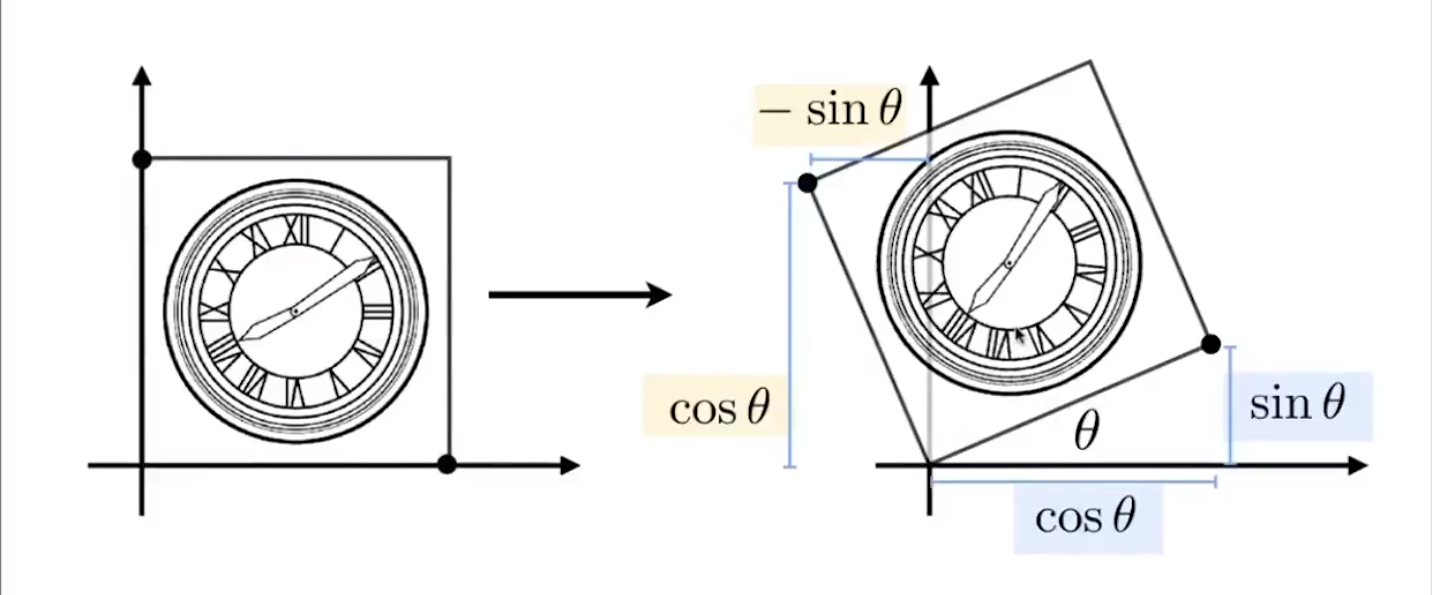
\includegraphics[scale=0.25]{resources/rotateMatrixGraphics.png}

    因此二维的旋转矩阵$$
      R_\theta = \begin{bmatrix}
        \cos\theta & -\sin\theta \\
        \sin\theta & \cos\theta
      \end{bmatrix}
    $$


    \section{齐次坐标}{
      由于单纯的线性变换并不能让对象动起来,依然只能在原点操作,所以需要齐次坐标表示空间上的位移.

      如下图:

      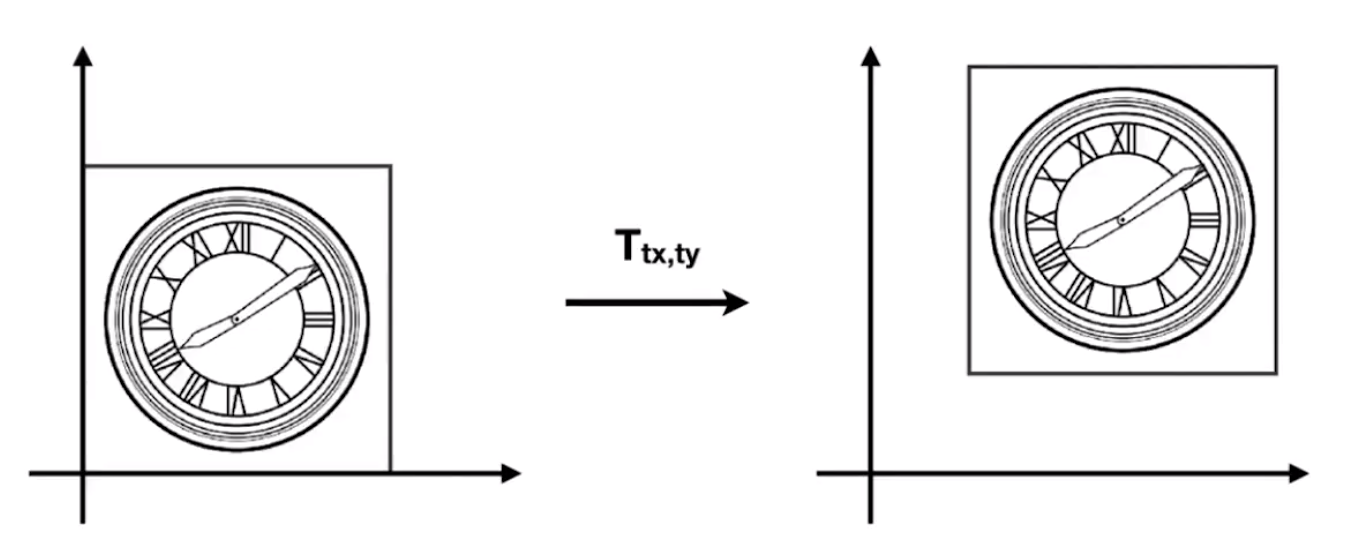
\includegraphics[scale=0.25]{resources/homogeneous_coordinates.png}

      用$x\prime$和$y\prime$来表示变换后的坐标,公式为:

      $x\prime = x + t_x$

      $y\prime = y + t_y$

      仔细思考一下发现似乎并不能写成矩阵$A\vec{x} = \vec{b}$的形式.

      事实上应该写成这样:
      $$
        \begin{bmatrix}
          x\prime \\
          y\prime
        \end{bmatrix}
        =
        \begin{bmatrix}
          a & b \\
          c & d
        \end{bmatrix}
        \begin{bmatrix}
          x \\
          y
        \end{bmatrix}
        +
        \begin{bmatrix}
          t_x \\
          t_y
        \end{bmatrix}
      $$

      因此平移变换不属于线性变换.但是人们不想要特殊情况,于是引入了齐次坐标:

      还是拿二维的情况举例,增加一个维度,将二维的点表示为:
      $$\begin{bmatrix}
          x & y & 1
        \end{bmatrix}^T$$

      将二维向量表示为:
      $$\begin{bmatrix}
          x & y & 0
        \end{bmatrix}^T$$

      也就是说:再多增加一个维度用于说明表示的是一个点还是一个向量,这是因为向量具有平移不变性,不管怎么移动表示的始终是一个方向.

      齐次坐标的好处就在这里,它是这么用的:

      $$\begin{bmatrix}
          x\prime \\
          y\prime \\
          w\prime
        \end{bmatrix}
        =
        \begin{bmatrix}
          1 & 0 & t_x \\
          0 & 1 & t_y \\
          0 & 0 & 1
        \end{bmatrix}
        \cdot
        \begin{bmatrix}
          x \\
          y \\
          1
        \end{bmatrix}
        =
        \begin{bmatrix}
          x + t_x \\
          y + t_y \\
          1
        \end{bmatrix}
      $$

      更直观一点:可以这么理解:
      \begin{itemize}
        \item 向量 + 向量 = 向量, 向量相加还是向量 $0 + 0 = 0$
        \item 点 - 点 = 向量, 两点相减得到向量 $1 - 1 = 0$
        \item 点 + 向量 = 点, 一个点加一个向量结果是一个点 $0 + 1 = 1$
        \item 点 + 点 = 两个点的中点, $1 + 1 = 2$,原因见扩充定义.
      \end{itemize}
      扩充定义如下:
      $$\begin{bmatrix}
          x \\
          y \\
          w
        \end{bmatrix} = \begin{bmatrix}
          x \\
          y \\
          w
        \end{bmatrix}\cdot\cfrac{1}{w} = \begin{bmatrix}
          \cfrac{x}{w} \\
          \cfrac{y}{w} \\
          1
        \end{bmatrix}$$

      {\bfseries于是总结,给出以下下定义:}\\\\\indent
      仿射变换(Affine transformation) = 线性变换(Linear transformation) + 位移(transformation)

      即:
      $$\begin{bmatrix}
          x\prime \\
          y\prime
        \end{bmatrix}
        =
        \begin{bmatrix}
          a & b \\
          c & d
        \end{bmatrix}
        \cdot
        \begin{bmatrix}
          x \\
          y
        \end{bmatrix}
        +
        \begin{bmatrix}
          t_x \\
          t_y
        \end{bmatrix}$$

      都可以写成齐次坐标(homogeneous coordinates)的形式

      即:
      $$\begin{bmatrix}
          x\prime \\
          y\prime \\
          1
        \end{bmatrix}
        =
        \begin{bmatrix}
          a & b & t_x \\
          c & d & t_y \\
          0 & 0 & 1
        \end{bmatrix}
        \cdot
        \begin{bmatrix}
          x \\
          y \\
          1
        \end{bmatrix}$$

      {\bfseries不如直接将其他操作的齐次坐标形式补全吧?}
      \begin{itemize}
        \item 缩放(scale) : $$S(s_x, s_y) = \begin{bmatrix}
                  s_x & 0   & 0 \\
                  0   & s_y & 0 \\
                  0   & 0   & 0
                \end{bmatrix}$$
        \item 旋转(rotation) : $$R(\alpha) = \begin{bmatrix}
                  \cos\alpha & -\sin\alpha & 0 \\
                  \sin\alpha & \cos\alpha  & 0 \\
                  0          & 0           & 1
                \end{bmatrix}$$
        \item 平移(translation) : $$T(t_x, t_y) = \begin{bmatrix}
                  1 & 0 & t_x \\
                  0 & 1 & t_y \\
                  0 & 0 & 1
                \end{bmatrix}$$
      \end{itemize}

     }%齐次坐标结尾

    \subsection{组合变换}{
      可以通过组合各个基础变换以形成复杂的变换效果.

      组合方法为对应矩阵按照顺序从右向左做乘法.

      大部分时候组合顺序至关重要.

    }%组合变换结尾

    \subsection{三维变换}{
      以上结论都可以用于三维,推而广之:\\

      齐次坐标:\begin{itemize}
        \item 三维点:$$\begin{bmatrix}
                  x \\
                  y \\
                  z \\
                  1
                \end{bmatrix}$$
        \item 三维向量:$$\begin{bmatrix}
                  x \\
                  y \\
                  z \\
                  0
                \end{bmatrix}$$
      \end{itemize}

      $\left[x\ y\ z\ w\right]^T$,当$w$不等于$1$他所表示的三维的点其实是(第四个维度已略去):
      $$\begin{bmatrix}
          \cfrac{x}{w} \\
          \cfrac{y}{w} \\
          \cfrac{z}{w} \\
        \end{bmatrix}$$

      同样的,三维空间中齐次坐标描述的仿射变换的矩阵是$4 \times 4$的:
      $$\begin{bmatrix}
          x\prime \\
          y\prime \\
          z\prime \\
          1
        \end{bmatrix}
        =
        \begin{bmatrix}
          a & b & c & t_x \\
          d & e & f & t_y \\
          g & h & i & t_z \\
          0 & 0 & 0 & 1
        \end{bmatrix}
        \cdot
        \begin{bmatrix}
          x \\
          y \\
          z \\
          1
        \end{bmatrix}$$

      将二维操作类比过来:

      \begin{itemize}
        \item 缩放 : $$
                S(s_x,s_y,s_z) =\begin{bmatrix}
                  s_x & 0   & 0   & 0 \\
                  0   & s_y & 0   & 0 \\
                  0   & 0   & s_z & 0 \\
                  0   & 0   & 0   & 1
                \end{bmatrix}
              $$
        \item 平移 : $$
                T(t_x,t_y,t_z) = \begin{bmatrix}
                  1 & 0 & 0 & t_x \\
                  0 & 1 & 0 & t_y \\
                  0 & 0 & 1 & t_z \\
                  0 & 0 & 0 & 1
                \end{bmatrix}
              $$
        \item 三维旋转(绕某个轴逆时针旋转) :
              $$
                R_x(\alpha) = \begin{bmatrix}
                  1 & 0          & 0           & 0 \\
                  0 & \cos\alpha & -\sin\alpha & 0 \\
                  0 & \sin\alpha & \cos\alpha  & 0 \\
                  0 & 0          & 0           & 1
                \end{bmatrix}
              $$

              $$
                R_y(\alpha) = \begin{bmatrix}
                  \cos\alpha  & 0 & \sin\alpha & 0 \\
                  0           & 1 & 0          & 0 \\
                  -\sin\alpha & 0 & \cos\alpha & 0 \\
                  0           & 0 & 0          & 1
                \end{bmatrix}
              $$

              $$
                R_z(\alpha) = \begin{bmatrix}
                  \cos\alpha & -\sin\alpha & 0 & 0 \\
                  \sin\alpha & \cos\alpha  & 0 & 0 \\
                  0          & 0           & 1 & 0 \\
                  0          & 0           & 0 & 1
                \end{bmatrix}
              $$
        \item 三维旋转(欧拉角) : $R_{xyz}(\alpha,\beta,\gamma) = R_x(\alpha)R_y(\beta)R_z(\gamma)$
        \item 三维旋转($\vec{I}$绕任意轴n旋转角度$\alpha$)(罗德里格斯旋转公式) : $$
                R(n,\alpha) = \cos(\alpha)\vec{I} + (1 - \cos(\alpha))\vec{n}\vec{n}\transpose + \sin(\alpha)\begin{bmatrix}
                  0    & -n_z & n_y  \\
                  n_z  & 0    & -n_x \\
                  -n_y & n_x  & 0
                \end{bmatrix}
              $$
              (其中$\vec{n}$为旋转轴的单位向量)
      \end{itemize}
    }%三维变换结尾

    \subsection{观测变换}{
      一般来说拍一张照片的步骤如下 :

      \begin{enumerate}
        \item 找到一个好的位置摆放人物(模型变换,model transformation)
        \item 找到一个好的"角度"来放下相机(视图变换,view transformation)
        \item 按下快门(投影变换,projection transformation)
      \end{enumerate}

      \begin{itemize}
        \item {
              视图变换(view transformation) :

              首先定义相机:
              \begin{itemize}
                \item 位置(Position) : $\vec{e}$
                \item 视线方向(Look-at/gaze direction) : $\hat{\vec{g}}$
                \item 向上方向(UP direction) : $\hat{\vec{t}}$ (注:这个表示的是相机自身的旋转,此向量垂直于上面两个向量张成的平面)
              \end{itemize}

              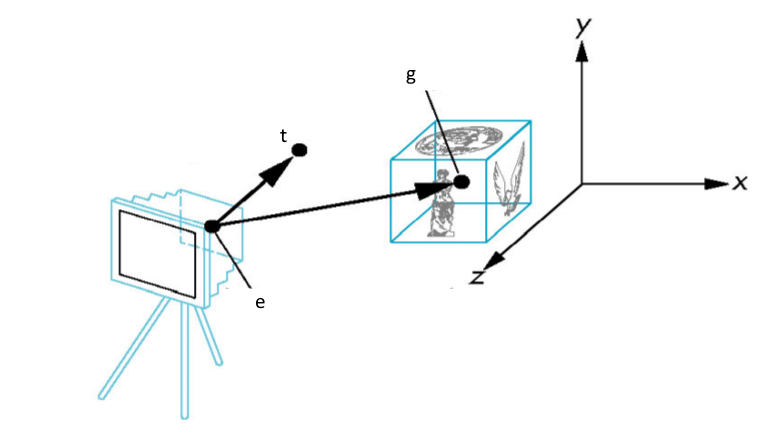
\includegraphics[scale=0.9]{resources/viewTransformation.png}

              值得注意的是: 定义相机永远在原点,视线朝向-z方向,以y轴作为向上方向(约定俗成,这么做有很多好处)

              所以在实际情况中,需要将相机和被观测的对象视作一个整体,进行如下操作:
              \begin{enumerate}
                \item 将$\vec{e}$平移到原点.
                \item 将$\hat{\vec{g}}$旋转到-z方向
                \item 将$\hat{\vec{t}}$旋转到y方向
                \item 将$\hat{\vec{g}} \times \hat{\vec{t}}$旋转到x方向
              \end{enumerate}

              这一系列的矩阵操作记作$M_{view}$,如下:

              \begin{itemize}
                \item 令$M_{view} = R_{view}T_{view}$
                \item 将$\vec{e}$平移到原点 : $$
                        T_{view} = \begin{bmatrix}
                          1 & 0 & 0 & -x_e \\
                          0 & 1 & 0 & -y_e \\
                          0 & 0 & 1 & -z_e \\
                          0 & 0 & 0 & 1
                        \end{bmatrix}
                      $$
                \item 将$\hat{\vec{g}}$旋转到-z方向,将$\hat{\vec{t}}$旋转到y方向,($\hat{\vec{g}} \times \hat{\vec{t}}$)旋转到x方向
                \item 仔细思考,发现上面的矩阵想要直接计算出来过于繁琐,应当反向思考—做基变换,再求逆以得到旋转矩阵 : $$
                        R^{-1}_{view} = \begin{bmatrix}
                          x_{\hat{\vec{g}} \times \hat{\vec{t}}} & x_{\hat{\vec{t}}} & x_{-\hat{\vec{g}}} & 0 \\
                          y_{\hat{\vec{g}} \times \hat{\vec{t}}} & y_{\hat{\vec{t}}} & y_{-\hat{\vec{g}}} & 0 \\
                          z_{\hat{\vec{g}} \times \hat{\vec{t}}} & z_{\hat{\vec{t}}} & z_{-\hat{\vec{g}}} & 0 \\
                          0                                      & 0                 & 0                  & 1
                        \end{bmatrix}
                        R_{view} = \begin{bmatrix}
                          x_{\hat{\vec{g}} \times \hat{\vec{t}}} & y_{\hat{\vec{g}} \times \hat{\vec{t}}} & z_{\hat{\vec{g}} \times \hat{\vec{t}}} & 0 \\
                          x_{\hat{\vec{t}}}                      & y_{\hat{\vec{t}}}                      & z_{\hat{\vec{t}}}                      & 0 \\
                          x_{-\hat{\vec{g}}}                     & y_{-\hat{\vec{g}}}                     & z_{-\hat{\vec{g}}}                     & 0 \\
                          0                                      & 0                                      & 0                                      & 1
                        \end{bmatrix}
                      $$
                      (由于旋转矩阵是正交矩阵,所以求逆等于求转置.)
              \end{itemize}
              随着相机的变换,其他所有物体也应当跟着变换,这样才能保证拍出来的是同样的照片.
              }

        \item {
              投影变换(projection transformation) :

              投影分为两种 : 正交投影(Perspective projection)和透视投影(Orthographic projection):

              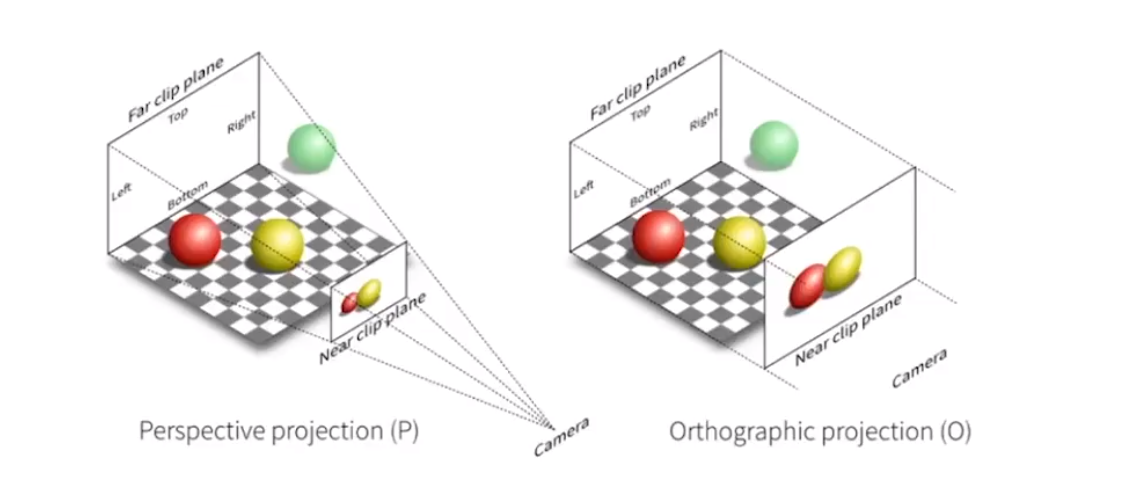
\includegraphics[scale=0.5]{resources/twoProjectionTransformation.png}

              两种投影的本质区别就在于是否有近大远小的现象.

              \begin{itemize}
                \item {
                      正交投影(Orthographic projection) :

                      先定义一个空间中的立方体, 给出三个轴的范围$[l,r]\times[b,t]\times[f,n]$,平移并缩放到标准立方体$[-1,1]^3$

                      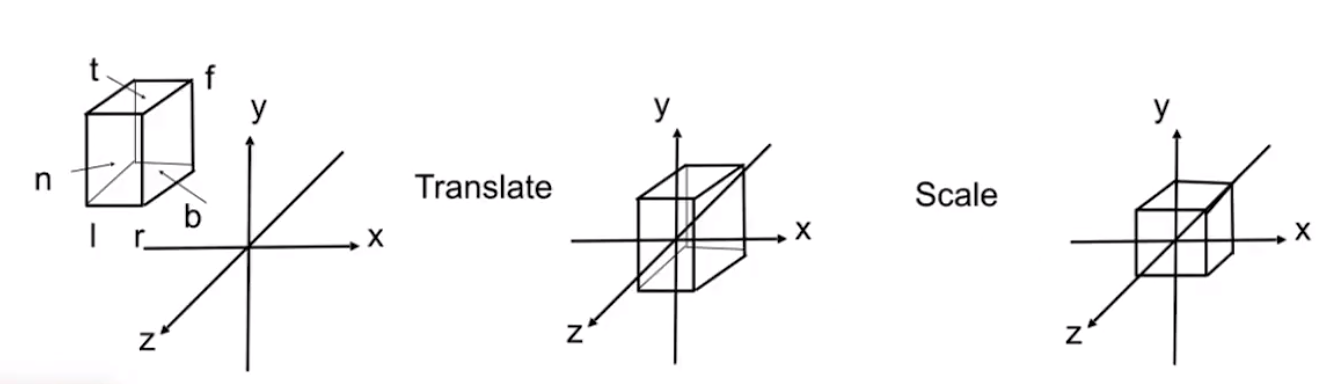
\includegraphics[scale=0.5]{resources/OrthographicProjection.png}

                      矩阵形式为:$$
                        M_{ortho} = \begin{bmatrix}
                          \cfrac{2}{r - l} & 0                & 0                & 0 \\
                          0                & \cfrac{2}{t - b} & 0                & 0 \\
                          0                & 0                & \cfrac{2}{n - f} & 0 \\
                          0                & 0                & 0                & 1
                        \end{bmatrix}
                        \begin{bmatrix}
                          1 & 0 & 0 & -\cfrac{r + l}{2} \\
                          0 & 1 & 0 & -\cfrac{t + b}{2} \\
                          0 & 0 & 1 & -\cfrac{n + f}{2} \\
                          0 & 0 & 0 & 1
                        \end{bmatrix}
                      $$

                      \begin{itemize}
                        \item 注意:由于视线方向沿着-z,所以$n>f$
                        \item 这就是为啥OpenGL用的是左手系
                      \end{itemize}
                      }
                \item {
                      透视变换(Perspective projection) :

                      首先把视锥压缩成长方体.(近平面永远不变,远平面z值不发生变化,中心点不发生变化)$(n \to n,f \to f,M_{persp \to ortho})$

                      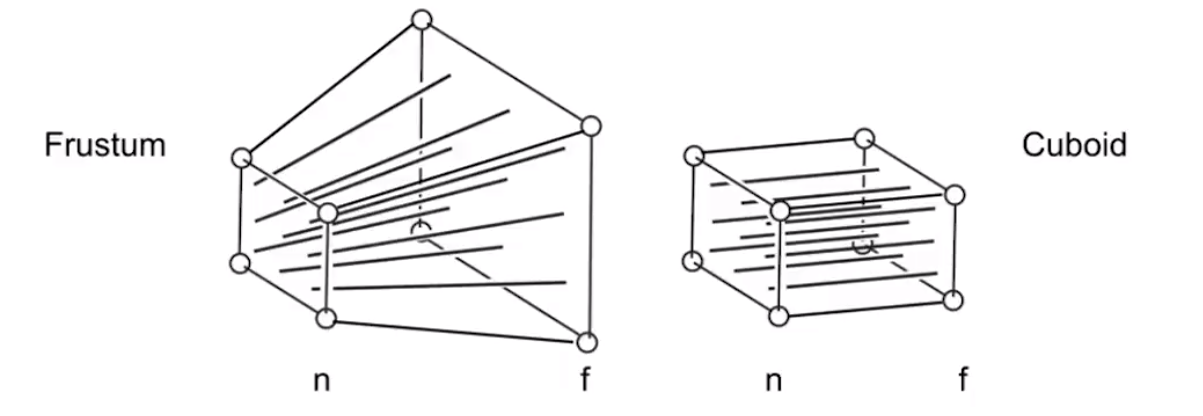
\includegraphics[scale=0.5]{resources/perspectiveProjection.png}

                      关键就在于:要找到中点和被投影对象之间的联系.

                      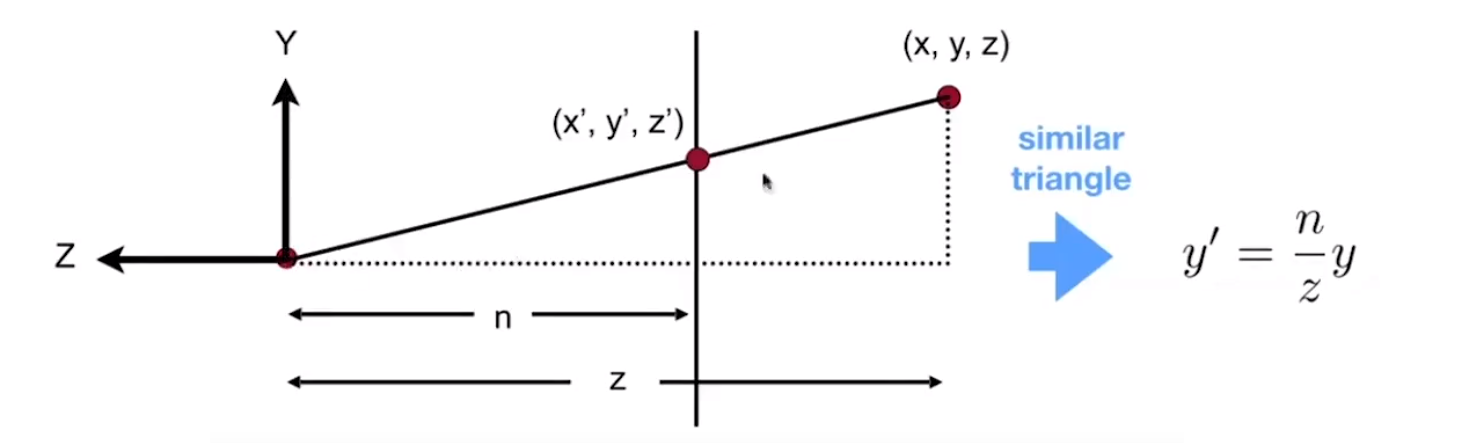
\includegraphics[scale=0.5]{resources/perspectiveProjection_middle.png}

                      $y^\prime = \cfrac{n}{z}y$,由这个公式就可以算出来压缩后的y,并且结果是满足要求的.

                      类似的,还有$x^\prime = \cfrac{n}{z}x$

                      于是得出结论:$$
                        \begin{bmatrix}
                          x \\
                          y \\
                          z \\
                          1
                        \end{bmatrix}
                        \Rightarrow
                        \begin{bmatrix}
                          \cfrac{nx}{z} \\
                          \cfrac{ny}{z} \\
                          unknow        \\
                          1             \\
                        \end{bmatrix}
                        ==
                        \begin{bmatrix}
                          nx           \\
                          ny           \\
                          still unknow \\
                          z
                        \end{bmatrix}
                      $$
                      因此,透视变换的本质就是由目标平面和被投影平面构造一个直角三角形

                      由此写出未完成的投影矩阵 : $$
                        M_{persp \to ortho}
                        =
                        \begin{bmatrix}
                          n & 0 & 0 & 0 \\
                          0 & n & 0 & 0 \\
                          ? & ? & ? & ? \\
                          0 & 0 & 1 & 0
                        \end{bmatrix}
                      $$

                      而这一行未知的也一定与z有关系.

                      另外,任何在目标平面上的点被投影后一定在原地,也就是说:$$
                        \begin{bmatrix}
                          x \\
                          y \\
                          n \\
                          1
                        \end{bmatrix}
                        \Rightarrow
                        \begin{bmatrix}
                          x \\
                          y \\
                          n \\
                          1
                        \end{bmatrix}
                        ==
                        \begin{bmatrix}
                          nx  \\
                          ny  \\
                          n^2 \\
                          n
                        \end{bmatrix}
                      $$

                      仔细思考可以得出:矩阵第三行前两个未知数一定为0:$$
                        \begin{bmatrix}
                          0 & 0 & A & B
                        \end{bmatrix}
                        \begin{bmatrix}
                          x \\
                          y \\
                          n \\
                          1
                        \end{bmatrix}
                        =
                        n^2
                      $$

                      结合另一件事 : 被投影平面上的中心点投影后位置不变,可得出:$$
                        \begin{cases}
                          \begin{bmatrix}
                            0 & 0 & A & B
                          \end{bmatrix}
                          \begin{bmatrix}
                            x \\
                            y \\
                            n \\
                            1
                          \end{bmatrix}
                          =
                          n^2
                          \rightarrow
                          An + B = n^2 \\
                          \begin{bmatrix}
                            0 \\
                            0 \\
                            f \\
                            1
                          \end{bmatrix}
                          \Rightarrow
                          \begin{bmatrix}
                            0 \\
                            0 \\
                            f \\
                            1
                          \end{bmatrix}
                          ==
                          \begin{bmatrix}
                            0   \\
                            0   \\
                            f^2 \\
                            f
                          \end{bmatrix}
                          \rightarrow
                          Af + B = f^2
                        \end{cases}
                        \rightarrow
                        \begin{cases}
                          A = n + f \\
                          B = -nf
                        \end{cases}
                      $$
                      所以 : $$
                        M_{persp \to ortho}
                        =
                        \begin{bmatrix}
                          n & 0 & 0     & 0   \\
                          0 & n & 0     & 0   \\
                          0 & 0 & n + f & -nf \\
                          0 & 0 & 1     & 0
                        \end{bmatrix}
                      $$

                      最后将正交投影和此式结合起来使矩阵变得完整 : $M_{persp} = M_{ortho}M_{persp \to ortho}$
                      }
              \end{itemize}
              }
      \end{itemize}

    }%观测变换结尾

   }%变换结尾

  \section{光栅化}{

    \subsection{定义与解释}{
      \begin{itemize}
        \item {
              什么是屏幕?
              \begin{itemize}
                \item 对于图形学来说,抽象的认为是一个二维数组,其中每一个元素都是一个像素.
                \item 数组的大小 : 分辨率.
                \item 一个典型的光栅(raster)成像设备.
              \end{itemize}
              }
        \item{
              什么是光栅(raster)?
              \begin{itemize}
                \item raster是德语中"屏幕"的意思.
                \item Rasterize-光栅化 == 把东西画到屏幕上.
              \end{itemize}
              }
        \item{
              像素(Pixel,"picture element"的缩写)是什么?
              \begin{itemize}
                \item 一个很小的只有单个颜色的方块.
                \item 颜色由不同比例的三原色(红绿蓝,rgb)混合而成.
              \end{itemize}
              }
        \item{
              关于"屏幕空间(screen space)"的定义

              \begin{center}
                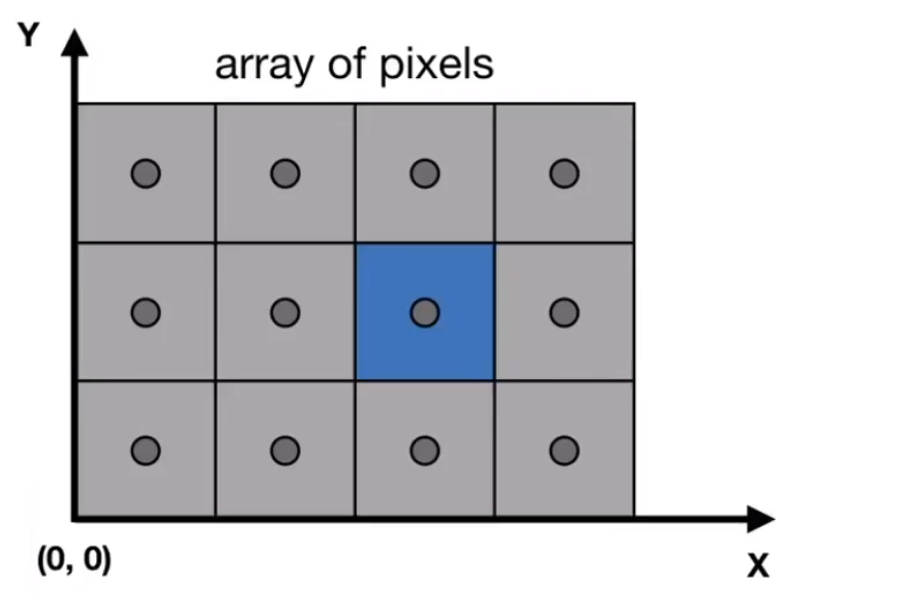
\includegraphics[scale=0.5]{resources/define_of_screen_space_1.png}
              \end{center}

              \begin{itemize}
                \item 认为屏幕的左下角是原点,向上是Y,向右是X.
                \item 像素的坐标都是用$(x,y)$描述的,$x,y$是整数.
                \item 像素的下标范围是从$(0,0)$到$(width - 1,height - 1)$.
                \item 像素的中心总是位于$(x + 0.5,y + 0.5)$.
                \item 屏幕被覆盖到的范围是从$(0,0)$到$(width,height)$(全部铺满).
              \end{itemize}
              }
        \item{
              采样:
              \begin{itemize}
                \item 给定一个函数,在多个地方判断输出结果.
              \end{itemize}
              }
      \end{itemize}
    }%定义与解释结尾

    \subsection{三角形光栅化}{
      为什么是三角形?
      \begin{itemize}
        \item 三角形是最基础的多边形.
        \item 任何多边形都可以拆成三角形.
        \item 内部一定是个平面图形.
        \item 内外位置定义清晰
        \item 方便的渐变效果
      \end{itemize}

      将一个三角形光栅化最简单的做法:采样

      采样在图形学中是个重要的概念.此处所指的采样时值对屏幕空间中的像素中心进行采样.(即:判断像素中心是否在函数内,如果是就给像素涂色) :

      \begin{center}
        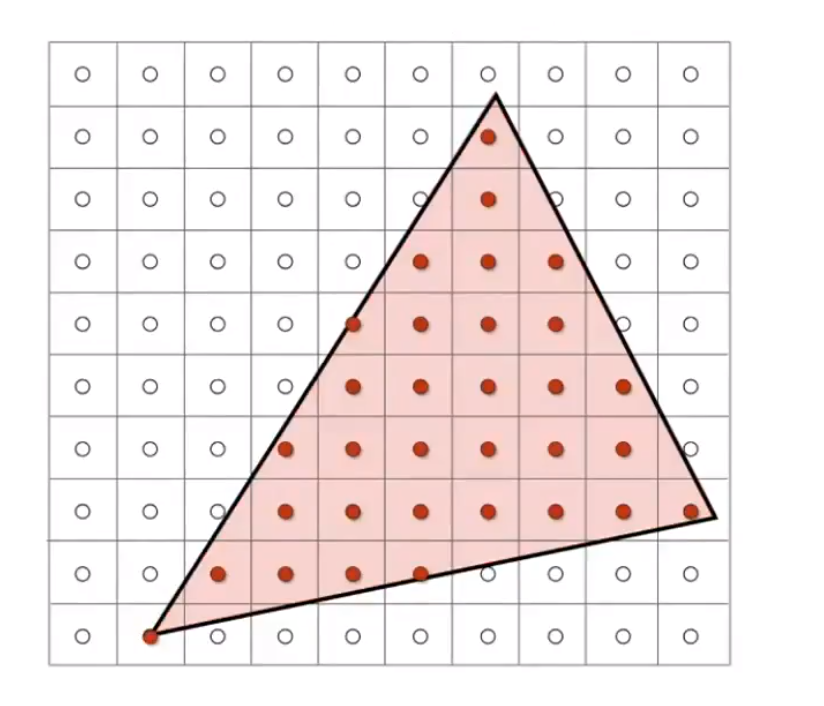
\includegraphics[scale=0.5]{resources/sample_if_each_pixel_inside_triangle.png}
      \end{center}

      代码实现很简单,两层循环遍历屏幕上所有的像素就行.

      要判断一个点是否在三角形内,只需要做叉乘 :

      \begin{center}
        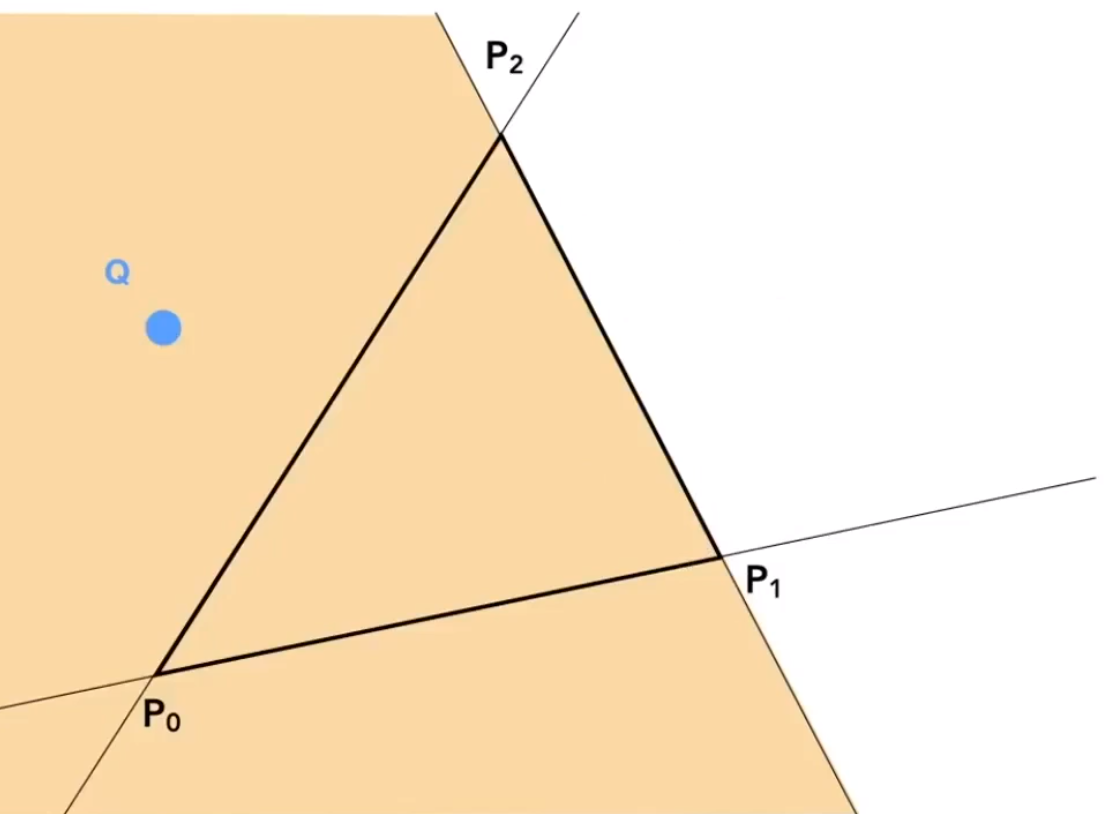
\includegraphics[scale=0.5]{resources/Triangle_Side_Cross_Prodyct.png}
      \end{center}

      比如:
      $$
        \vec{V_1} = \vec{P_1P_2} \times \vec{P_1Q}
      $$

      由于$\vec{V_1}$指向外侧,所以Q在$P_1P_2$左侧

      如此就能不断缩小范围,三条边都判断一次,就能知道该点是否在外面.

      如果点正好在边上,就自己决定.

      但是这么做性能消耗过大,因此可以界定一个判断范围-axis aliged bounding box :

      \begin{center}
        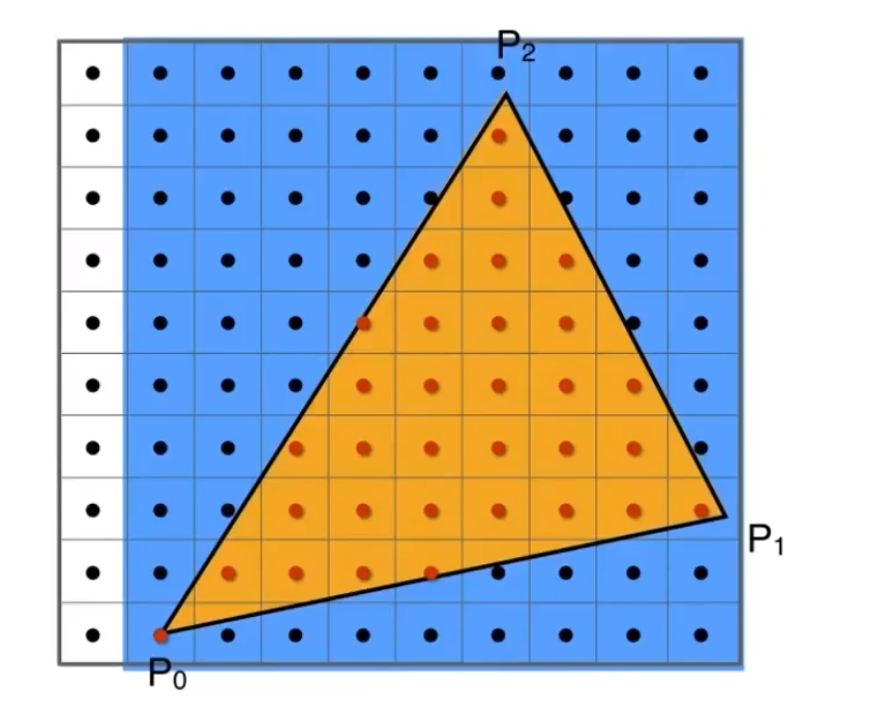
\includegraphics[scale = 0.5]{resources/pixel_boundingBox.png}
      \end{center}

      不过对不同的情况有不同的处理方法,优化方法百花八门,交给数据结构与算法篇吧.
    }%三角形光栅化结尾

   }%光栅化结尾

 }%计算机图形学结尾